\section{P,NP,NP-Completeness}
\subsection{Basic Concepts}
We have the following important definitions:
\begin{enumerate}
\item \textbf{Decision Problems}: those with output yes or no. \\
Technically, a decision problem is a function $f: \sum ^* \leftarrow \{0,1\}$, where $\sum^*=\bigcup _{n=0}^\infty \sum^n$, where $\sum^n$ is the set of all strings using alphabets in $\sum$ with length n, $x\in \sum^*$ is an instance.
\item \textbf{$\mathcal{P}$}: A problem is in $\mathcal{P}$ (usually easy) iff. it can be solved \textbf{polynomially}. \\
Technically, there is a \textbf{polynomial} algorithm $\mathcal{A}$, such that $\mathcal{A}(x)=f(x)$ holds, or there exists a polynomial time TM $\mathcal{A}(x)$ (always terminates within $p(|x|)$ steps) that outputs the correct answer.

$\mathcal{NP}$: Problems whose 'yes instance'(also called certificate) can be easily verified if a hint(an assignment of variables) is given, and any 'no instance' cannot be varified as 'yes'. (In test, you can just provide a certificate, and the others are straight forward)

\item \textbf{$\mathcal{NP}$-Hard}: All other $NP$ problems can reduce to such problem, but they may not be in $\mathcal{NP}$. \\NP-hardness can describe optimization problems, e.g. Maximum Independent Set is NP-hard

\textbf{$\mathcal{NP}$-Completeness}: The hardest problems in $\mathcal{NP}$, which are at least as hard as any other problem in $\mathcal{NP}$, or other problems reduce to them, $A \rightarrow NPC$.\\
 For decision problems: NP-complete = NP-hard + (in NP)

\textbf{ $\mathcal{NP}$-Intermediate}: Problems between $\mathcal{P}$ and $\mathcal{NP}$-Complete, with no natural examples, (since we haven't proven $P=NP$ yet)
\item \textbf{Reduction:} $A\rightarrow B$ means (karp) reduction from A to B; a mapping from A to B (see fig \ref{fig:reduction}); $A \leq _k B$, B is harder than A; use B to construct A; input instance I, if A(I)=1, then B(I)=1; if A(I)=0, then B(I)=0. See fig \ref{fig:reduction}.
 
\begin{figure}[htbp]
    \centering
    \begin{minipage}{0.45\linewidth}
        \centering
        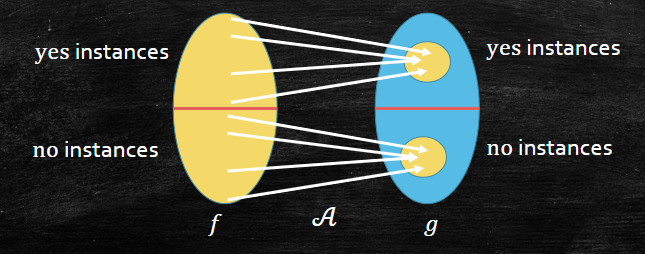
\includegraphics[width=0.8\linewidth]{Notes/fig/reduction.png}
        \caption{Reduction in Mapping's View}
        \label{fig:reduction}
    \end{minipage}
    %\qquad
    \begin{minipage}{0.5\linewidth}
        \centering
        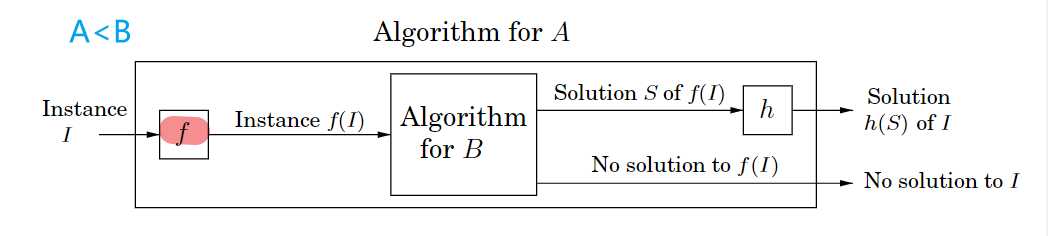
\includegraphics[width=1\linewidth]{Notes/fig/reduction_2.png}
        \caption{Reduction in algorithm's View: Key is to see B as a 'solver'}
    \end{minipage}
\end{figure}

\item \textbf{Turing Machine}: state diagram with a tape; what the pointer reads at present determines the next state; special states: starting, halting (accept, reject). see fig \ref{fig:turing}
\begin{figure}
    \centering
    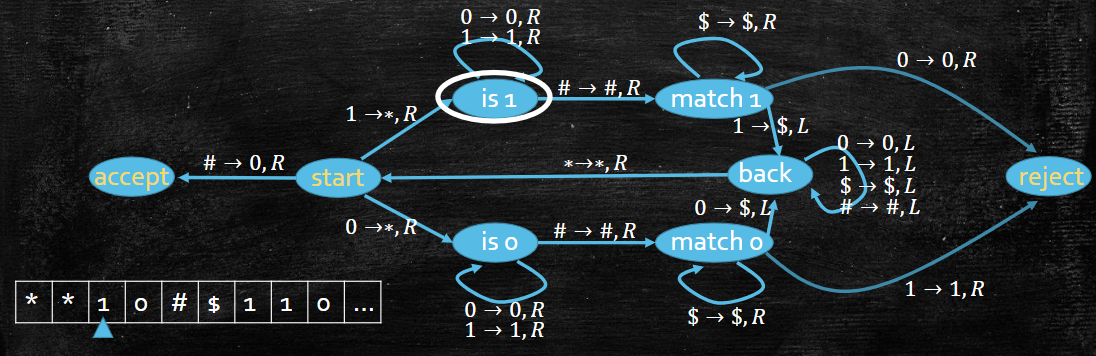
\includegraphics[width=0.7\linewidth]{Notes/fig/turing.png}
    \caption{Given x,y with the same length, check whether they are identical; the lower pipeline checks whether the both strings are at 1, and the higher pipeline checks whether the both strings are at 0.}
    \label{fig:turing}
\end{figure}
\end{enumerate}


Examples for problems in $\mathcal{P}$:
\begin{itemize}
    \item \textbf{Path:} Given a directed graph G and two vertices s and t, decide if there is a path from s to t.
    \item \textbf{k-flow:} Given a directed graph G, two vertices s and t, and flow capacity, decide if there is a path from s to t with at least k edges.
    \item \textbf{Prime:} Given n encoded in binary string, decide if n is a prime number.
\end{itemize}

\begin{prf}$P\subseteq NP$

If a decision problem is in $P$, there exists polynomial algorithm $\mathcal{A}$ s.t. $A(x)=y$. If it is in $NP$, its output can be verified in polynomial time. We verify the answer through feeding input $x$ into $A$ directly, i.e. through algorithm $A'(x,c)=A(x)$.  If $f(x)=1$, then $\exists y$ s.t. $A'$ accepts (x,y). If $f(x)=0$, then $\forall y, A'$ rejects (x,y). Thus, $f \in A'$.
\end{prf}

\subsection{5 NP-Completeness Problems}
We will prove that following examples are all NP problems as they reduce to each other.
First prove the pipeline in fig \ref{fig:NP}. The other way round is proven by Cook-Levin Theorem.

\begin{figure}
    \centering
    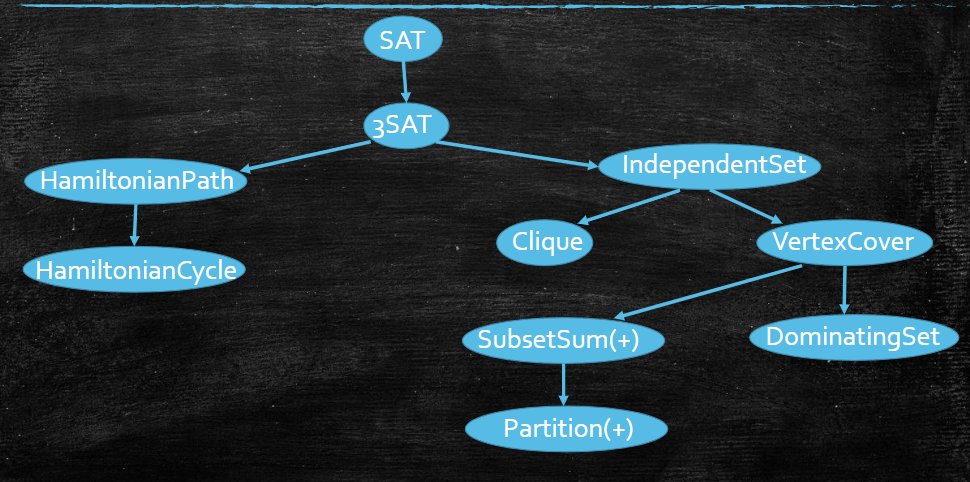
\includegraphics[width=0.8\linewidth]{Notes/fig/pipeline_for_NP.png}
    \caption{pipeline of our proof}
    \label{fig:NP}
\end{figure}
\begin{itemize}
    \item SAT[$\phi$]:
    Boolean Satisfiability Problem, given a CNF(conjunctive normal form: 'AND' of many clauses of 'OR', i.e.$\phi=(x_1 \lor x_2) \land (x_3 \lor \neg x_4) \land (\neg x_1 \lor \neg x_4)$)\\
    Reject if x does not encode a CNF formula $\phi$ or $y$ does not encode a valid Boolean assignment; Check if $y$ makes $\phi$ evaluated to true. Accept if it does, and reject if it does not

    \item Vertex Cover[$G=(V,E), k \in Z^+$]: Given an undirected unweighted graph G, decide if the graph has a vertex cover(contains at least a vertice of each edge) of
    size k.
    \item Independent Set[$G=(V,E),k \in Z^+$]: decide if the graph has an independent set(at most a vertice of each edge is chosen) of size k.
    \item Subset Sum[$S=\{a_1,\ldots,a_n\},k \in \mathcal{Z}^+$]: Decide if there is a sub-collection $T \subseteq S$ such that $\sum_{a_1 \in T}a_i=k$
    \item Hamiltonian Path[$G=(V,E)$]: Given an undirected graph, decide whether it contains a Hamiltonian path (longest path; path containing each vertex exactly once).
    % \item Clique: Given an undirected graph (G=(V,E)), decide whether it contains a clique of size k (complete subgraph with k vertices).
\end{itemize}


\begin{itemize}
\item $SAT\rightarrow 3SAT$\\
    We transfer SAT expression into 3-SAT by introducing a connector $y_i$:
\[x_1 \lor x_2 \lor \neg x_3 \lor \neg x_4= (x_1 \lor x_2 \lor y_1) \land \neg y_1 \lor \neg x_3 \lor \neg x_4\]
\item $3SAT\rightarrow$ Independent Set\\
    Construct Independent Set graph $G'$ from 3-SAT formula $\phi$:
    \begin{itemize}
        \item For each variable $x_i$, construct a triangle $T_i$ with vertices $x_i, \neg x_i, y_i$.
        \item For each clause $C_j$, add a vertex $z_j$ and connect it to all vertices in $T_i$ corresponding to literals in $C_j$.
        \item Set $k=m$, where $m$ is the number of clauses in $\phi$.
    \end{itemize}
    If $\phi$ is a yes instance, each clause must have a literal with value true. Pick exactly one vertex representing a true literal. Since S is an independent set, $|S|=k$, so $g(G,k)=1$
    If $\phi$ is a no instance, assume (G,m) is a yes instance. By triangle, you choose \textbf{exactly} one vertice in every triangle. Assigning true to literals representing the chosen vertices, and assign random value to others produces a certificate for 3-SAT.
\item Independent Set $\rightarrow$ Vertex Cover

    The complement of Independent Set is Vertex Cover. 
\item Vertex Cover $\rightarrow$ SubsetSum (VertexCover $\rightarrow$ VectorSubsetSum $\rightarrow$ SubsetSum)
\begin{itemize}
    \item Vertex Cover$\leq_k$ VectorSubsetSum 
    
    See \ref{fig:vertex_cover} for the construction.
        \begin{figure}
            \centering
            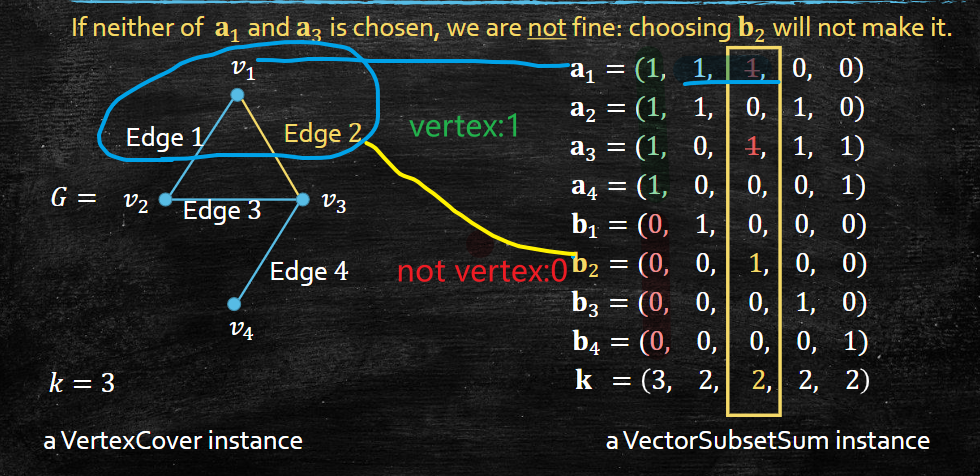
\includegraphics[width=0.6\linewidth]{Notes/fig/VSS.png}
            \caption{Vertex Cover $\leq_k$ VectorSubsetSum. Simple put, column sum=2 under such construction only implies that at least a vertice in each edge is chosen.}
            \label{fig:vertex_cover}
        \end{figure}
    \item VectorSubsetSum$\leq_k$ SubsetSum
    
    We can convert a vector $a=(a[0],\ldots, a[m])$ to a large number by a large enough base that avoids carry, so each vector is uniquely represented by a number. Additions with vectors are now equivalent to additions with numbers.
\end{itemize}
\item SubsetSum $\rightarrow$ Partition
Given subsetsum problem (S,k). Suppose it is a 'yes' instance, denote sum(S)=s $\sum_{i<m} a_i=k$, $\sum_{m\leq i\leq k} a_i=s-k$. We hope $\sum_{m\leq i\leq k} + b =k$, $b=2k-s$
\item 3SAT $\rightarrow$ Hamiltonian Path*
    \begin{itemize}
    \item 3SAT $\leq _k$ Directed Hamiltonian Path
    \begin{figure}
        \centering
        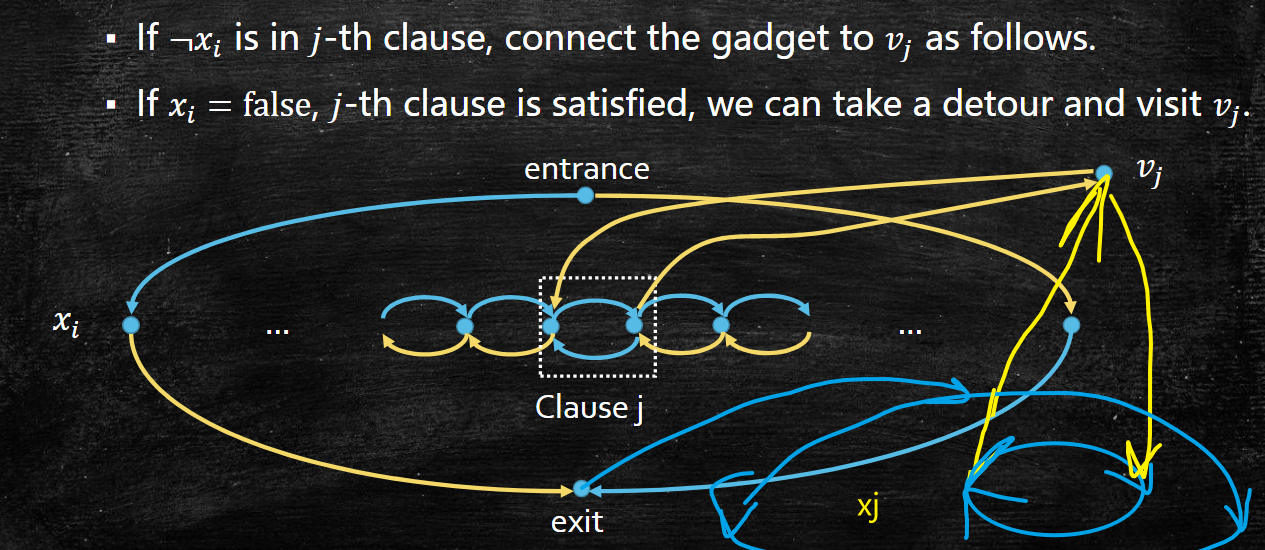
\includegraphics[width=0.6\linewidth]{Notes/fig/sat_dhp.png}
        \caption{3SAT $\leq _k$ Directed Hamiltonian Path}
        \label{fig:3SAT}
    \end{figure}
    If $\phi$ has a yes instance, we will prove that there exists a Hamiltonian path staring from s to t: For each clause, choose a representative true literature.
    Go from s to t, and visit each $v_j$ from its representative by
    taking a detour
    Prove the other way by contrapositive. If the graph has a Hamiltonian path, then $\phi$ is a yes instance. Each $v_j$ has to be visited by a detour from a variable
    \item Directed Hamilton Path $\leq _k$ Hamiltonian Path
    \begin{figure}
        \centering
        \includegraphics[width=0.6\linewidth]{Notes/fig/dhp_hp.png}
        \caption{Directed Hamiltonian Path $\leq _k$ Hamiltonian Path}
        \label{fig:dhp_hp}
    \end{figure}
\end{itemize}
\item Hamiltonian Path $\rightarrow$ Hamiltonian Cycle
\item By Cook-Levin Theorem, SAT is NP-complete, so they are all NP-complete.

In essense, the theorem proves that a CNF formula is sufficient to simulate the execution of a Turing Machine. See \ref{fig:}. For the neighbouring rows, the content differs by one bit. Since the TM operates in polynomial time, the number of columns are polynomial. Then the change can be computed in 'clause', so a CNF formula is sufficient to simulate the execution of a Turing Machine.
\end{itemize}


% Partition Partition+
% Hamiltonian Path, Directed Hamiltonian Path
% 3SAT< Directed Hamiltonian Path < Hamitonian Path
% n literals, m clauses
% If $x_i$ = true, j-th clause is satisfied, we can take a detour and visit $v_j$. If $\neg x_i$ is in j-th clause, construct the path the opposite way.
% % figure

% Directed Hamiltonian Path < Hamitonian Path
% If you go in and out on yellow edge, then you will never visit $u^{mid}$. Vertice gadget % figure

% Lemma 1. The path in 𝐺′ must start at 𝑠𝑖𝑛 and end at 𝑡𝑜𝑢𝑡.
% ▪ Lemma 2. If we first enter a vertex gadget at 𝑢𝑖𝑛 (or 𝑢𝑜𝑢𝑡)
% we must proceed to 𝑢𝑚𝑖𝑑 and then to 𝑢𝑜𝑢𝑡 (or 𝑢𝑖𝑛)
% The pattern of the path must be 𝑖𝑛 → 𝑚𝑖𝑑 →
% 𝑜𝑢𝑡 → 𝑖𝑛 → 𝑚𝑖𝑑 → 𝑜𝑢𝑡 → ⋯
\subsection{Summary of a NP Completeness Proof}
\begin{enumerate}
    \item Prove $f \in NP$.
    \item Construct the reduction $g \leq _k f$.
    For a fixed instance x of g. Design transfer function $\phi$, $y=\phi(x)$.
    \item (Completeness) x is yes $\rightarrow$ y is yes
    \item (Soundness) x is no $\rightarrow$ y is no. 
    Or, proving the contrapositive “y is yes $\rightarrow$ x is yes” is often easier.
\end{enumerate}    
